\chapter{Curriculum Learning}

Like most of the terms, ML research borrowed ‘Curriculum Learning’ from cognitive science. Curriculum learning draws a parallel from human intelligence to machine intelligence. As humans learn through meaningfully ordered, sophisticated education system, machines can also profit from guided learning patterns \cite{Bengio2009}. In fact, Elman demonstrates how starting small in both human and machine context results in enhanced learning \cite{Elman1993}. He designed a recurrent neural network to learn a grammatical structure of a language. This model at the beginning of the training had limited and restrictive capacity, later on gained more resources to exploit. Akin to a toddler, who has limited cognitive ability but manages to learn a language fluently. Elman’s approach proved to understand a grammatical structure of a language, which, without the curriculum approach, would be impossible to comprehend. In general, either in human or machine setting, curriculum learning promises faster convergence and better generalization \cite{Bengio2009}. 

Curriculum learning also unlocks new possibilities in robot learning. Indeed, Sanger showed inverse dynamics problem on robotics manipulators could be solved with the integration of Trajectory Extension Learning \cite{Sanger1994}. During training, he commands an approximate solution for the next value of parameters as guidance \cite{Sanger1994}. Karpathy et al. evaluated a two-level curriculum structure to learn the motor skills of the acrobat. He showed that curriculum learning could bring enhanced generalization of learned skills for underactuated control \cite{Karpathy2012}. Consequently, Breyer et al., before our work, have proved that the curriculum learning approach can facilitate the learning of a robotics manipulator on object grasping tasks. They found the curriculum integrated trials the most successful \cite{Breyer2018}.

\begin{figure}[htbp]
    \centering
      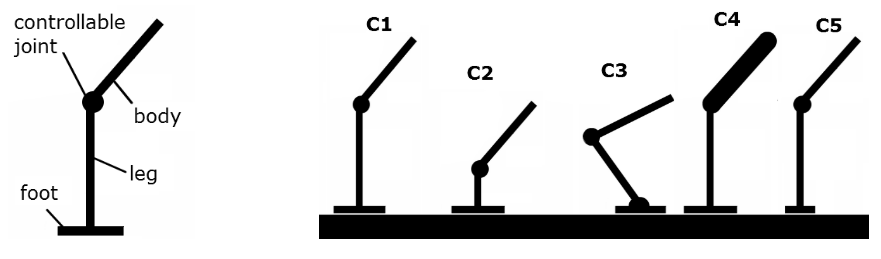
\includegraphics[width=0.9\textwidth]{figures/acrobot}
    \caption{Acrobot learned motor skills through two-level curriculum strategy \cite{Karpathy2012}}
    \label{fig:curriculum}
\end{figure}

Either on supervised learning or reinforcement learning, curriculum integration proved to be useful to ease the learning process. Even though curriculum strategy brings a high number of hyperparameters and prior bias from expert knowledge, we found curriculum learning as the most critical part of our work. As we represent in the future work section, we believe the automatic learning of curriculum parameters will bring more attention to the curriculum-based techniques.
